\documentclass{article}
\usepackage{tikz}
\usetikzlibrary{calendar}
\usepackage{amsmath}
\usepackage[utf8]{inputenc}

\title{Rapport intermediaire pour Projet Long}
\author{Nicolas Peneloux, Ymri Scheiner}
\date{15 Mars 2024}

\begin{document}

\maketitle

\section{Introduction}

Notre projet consiste à réaliser un autotuner, c'est-à-dire un programme qui reçoit en entrée un fichier audio d'une voix, et ressort en sortie une version de cet audio dont les notes sont modifiées selon les désirs de l'utilisateur, sans altérer le reste de l'audio. Grossièrement, nous pouvons diviser cela en deux :
\begin{itemize}
  \item Pitch Tracking : récupérer les différentes notes de l'audio
  \item Pitch Correction : changer les notes vers les hauteurs souhaitées
\end{itemize}
\par 

\subsection*{Métriques}
Pour mesurer le succès de notre projet, nous avons choisi une métrique de succès basée sur la distance entre les signaux de sortie produits par notre algorithme et ceux produits par une 
implémentation de référence. Plus précisément, nous définissons la mesure de succès comme suit :
\begin{equation}
    \operatorname{succes} = \max_{x \in \mathrm{entrees\_testees}} d(A(x), B(x))
\end{equation}
\par

où \( \mathit{A} \) et \( \mathit{B} \) représentent respectivement notre algorithme et l'implémentation de référence, \(\textit{d}\) est une fonction de distance entre les signaux audio, et \(\mathit{entrees\_testees}\) est un tableau contenant les fichiers audio d'entrée à tester.
\par
Nous définissons également un seuil maximal de distance autorisée entre les signaux de sortie de \(\textit{A}\) et \(\textit{B}\), noté \(\textit{seuil\_max}\). Si la mesure de succès est inférieur
à ce seuil, nous considérons que notre projet est réussi.

Pour calculer la mesure de succès, nous parcourons tous les signaux audio d'entrée dans le \( \textit{entrees\_testees} \). Pour chaque entrée, nous appliquons \( \textit{A} \) et \( \textit{B} \) pour produire deux signaux de sortie. Nous calculons ensuite la distance entre ces deux signaux de sortie à l'aide de \( \textit{d} \). Puis, nous mettons à jour la mesure de succès en prenant la valeur max entre la distance actuelle et la mesure de succès précédente.

Une fois que nous avons parcouru tous les signaux audio d'entrée, nous comparons la mesure de succès obtenue à notre seuil maximal \( \textit{seuil\_max} \). Si la mesure de succès est inférieure à ce seuil, on considère que le test est passé correctement.


\par





\section{Implémentation}

Nous réalisons ce projet en \textbf{Rust}, en nous appuyant sur \textbf{l'algorithme FFT (Fast Fourier Transform)} pour représenter l'audio sous une forme de données pragmatiques pour notre projet, une méthode très courante pour le traitement de signal. Nous utilisons également d'autres algorithmes basés sur cette technologie tels que l'algorithme PIN pour la correction de hauteur.
\par
En termes de modules ou packages, la structure interne du projet est très simple, avec un fichier par tâche, à utiliser dans un main. Nous utilisons quelques packages de Rust pour certaines tâches auxiliaires au projet, telles que la création de l'interface graphique, ou la manipulation/création de fichiers MIDI.

\section{Jalons}

\subsection{Tâches à Réaliser}

Nous avons divisé le projet dans sa globalité en trois tâches principales, à savoir 
\begin{itemize}
  \item L'implémentation de l'algorithme FFT pour permettre de transformer des fichiers audio en données utilisables
  \item L'implémentation du pitch tracking
  \item L'implémentation de la pitch correction
\end{itemize}

Viennent ensuite s'ajouter des tâches auxiliaires telles que la mise en place de tests, ou encore la création de l'interface graphique.

\subsection{Tâches Terminées}

Les deux première tâches parmis celles énumérées au-dessus ont été réalisés, ainsi que quelques tâches auxiliaires. Des tests ont été mis en place pour la partie FFT, et l'interface utilisateur a déjà été conçue.

\subsection{Organisation Temporelle}

Il manque ainsi la partie pitch correction et l'implémentation de tests pour la partie pitch tracking. 
\par
Idéalement, nous pouvons consacrer 2 semaines sur l'implémentations des tests et les semaines restantes pour coder la partie pitch correction.


\subsection*{Calendrier Visuel}


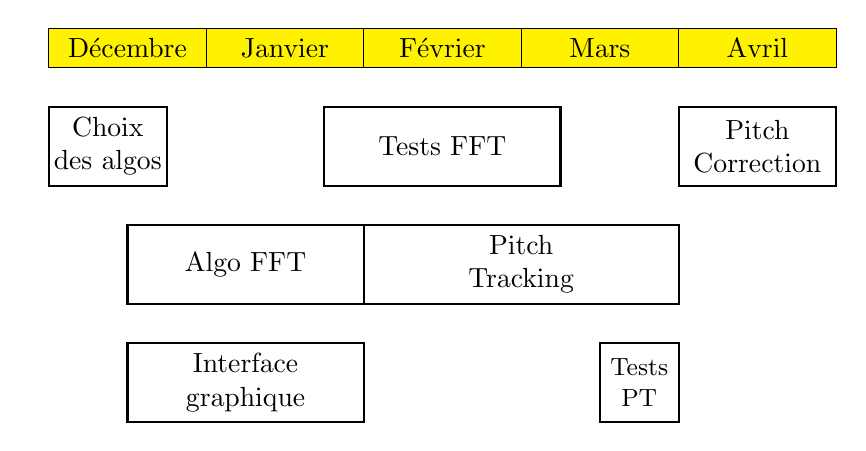
\begin{tikzpicture}
%Mois
\draw[fill=yellow] (0,0) rectangle (2,0.5) node[pos=.5] {Décembre};
\draw[fill=yellow] (2,0) rectangle (4,0.5) node[pos=.5] {Janvier};
\draw[fill=yellow] (4,0) rectangle (6,0.5) node[pos=.5] {Février};
\draw[fill=yellow] (6,0) rectangle (8,0.5) node[pos=.5] {Mars};
\draw[fill=yellow] (8,0) rectangle (10,0.5) node[pos=.5] {Avril};

%Tâches
\draw[thick] (0,-0.5) rectangle (1.5, -1.5) node[pos=.5, text width=1.8cm, align=center] {Choix des algos};
\draw[thick] (1,-2) rectangle (4, -3) node[pos=.5, text width=1.8cm, align=center] {Algo FFT};
\draw[thick] (1,-3.5) rectangle (4, -4.5) node[pos=.5, text width=1.8cm, align=center] {Interface graphique};
\draw[thick] (3.5,-0.5) rectangle (6.5, -1.5) node[pos=.5, text width=1.8cm, align=center] {Tests FFT};
\draw[thick] (4,-2) rectangle (8, -3) node[pos=.5, text width=1.8cm, align=center] {Pitch Tracking};
\draw[thick] (7,-3.5) rectangle (8, -4.5) node[pos=.5, text width=1cm, align=center, font=\small] {Tests PT};
\draw[thick] (8,-0.5) rectangle (10, -1.5) node[pos=.5, text width=1.8cm, align=center] {Pitch Correction};


\end{tikzpicture}

\section*{Problèmes rencontrés}
Nous avons d'abord mis du temps a trouver un sujet accepté, mais aussi après dans la réalisation du projet jusqu'a maintenant. Les difficultés majeures que nous avons rencontrées sont :
\begin{itemize}
  \item L'utilisation de Rust, que nous avons tout les deux dû apprendre pour le cadre de ce projet. Cela à rajouter d'avantage de retard pour le projet, il était assez difficile de commencer le projet
  sans avoir un minimum de base solide pour bien débuter.
  \item La compréhension théorique des algorithmes et technologies que nous utilisons. C'est, à tout les deux, notre premier projet dans le domaine du traitement audio.
  \item Le choix des algorithmes à utiliser. En rapport avec le point précédent, les différences peuvent être nuancées et dure a saisir sans en connaître les tenants et aboutissants. Certains algorithmes sont
  plus ou moins détailler, certains peuvent être même plutôt récent, et sans s'y connaître dans le domaine, on peut vite se retrouver perdu.
\end{itemize}

\end{document}
